\section{Deployment \label{deployment_section}}
\acrshort{ml} application has developed from being in domain of academic research to an applied field. A survey conducted by McKinsey \& Company \cite{analytics2019global} shows that nearly 25\% of business processes are adopting machine learning techniques. However, there is a huge difference and challenges to put ML in real world system as compared to academic settings. Reports from Algorithmia \cite{wiggers2019algorithmia, hecht2019add} shows that it takes 8 to 90 days for the majority of companies to deploy a single model and 18\% of companies took even more time to deploy. According to \acrfull{idc}'s report\footnote{\url{https://venturebeat.com/ai/idc-for-1-in-4-companies-half-of-all-ai-projects-fail/},Accessed: 22.03.2024} that includes 2,473 organizations into the survey, A notable portion has failed in an attempt of \acrshort{ai} deployments. Moreover, the \acrshort{idc}'s report points that the reasons could be lack of expertise, bias in data and high costs of resources.

When we talk about deploying ML functionality in production, there are several aspects that should be discuss such as machine learning deployment workflow, ethical considerations, law, end-user's trust, and security which are briefly discussed in \cite{paleyes2022challenges}. The term to make a service or a product using machine learning and making available for users refer as production. Sometimes the term ML deployment workflow also known as ML pipelines and there are various definitions and descriptions of it such as Cros-Industry Standard Process For Data Mining (CRISP-DM) \cite{shearer2000crisp} or Team Data Science Process (TDSP) \cite{TDSP}. In general, the process of developing machine learning based product and services in industrial environment have stages like data management, model learning, model verification and model deployment. Each of these stages can be further broken down in smaller steps as shown in \Cref{tab:deployment_stages} and each steps can run in parallel while informing each other through feedback loops. For developing ML pipelines, one could think of using best practices to use software development principles for productionizing machine learning products and services such as DevOps. It is about fast, flexible and provisioning business processes that integrates development, delivery and operations more efficiently thus pronounce as DevOps. It was an organizational shift from distributed groups or departments that performs function separately to cross-functional teams that works on continuous operational feature deliveries. These principles of DevOps brought a cultural shift towards in the collaboration between areas like development, quality assurance and operations. In paper \cite{ebert2016devops}, authors have presented a comprehensive case study of different tools and micro-services and the impact of these DevOps technologies on industry projects, An overall DevOps model's areas are shown in \Cref{fig:DevOps}. 

\begin{figure}[hb]
    \centering
    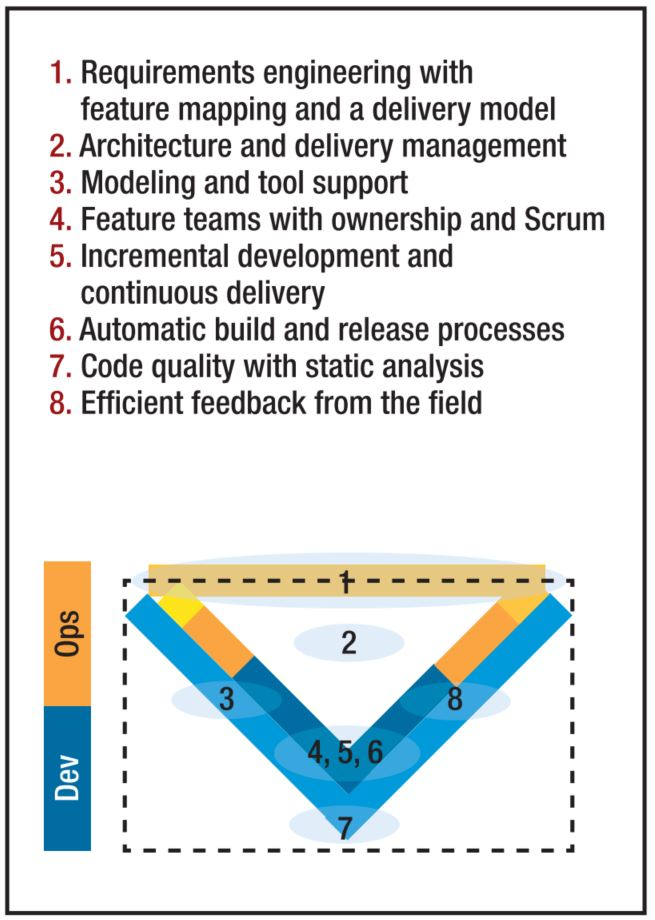
\includegraphics[width=0.45 \textwidth]{chapters/images/Literature_review/DevOps.JPG}
    \caption{A DevOps model infrastructure \cite{ebert2016devops}}
    \label{fig:DevOps}
\end{figure}

Some of these DevOps principles can be directly apply to ML systems but there are number of challenges that are specific to the machine learning, which are briefly discussed in \cite{dang2019aiops}, this paper introduced the term AIOps (also recognized as MLOps) that refer as DevOps tasks for ML systems. The market for machine learning services and tools is already started gaining growth. There are new tools and services being introduced continuously in order to overcome the problems in the deployment process. For example platforms like AWS SageMaker\footnote{\url{https://aws.amazon.com/sagemaker/},Accessed: 22.03.2024}, AzureML\footnote{\url{ https://azure.microsoft.com/en-us/products/machine-learning}, Accessed: 22.03.2024}, TensorFlow TFX\footnote{\url{https://www.tensorflow.org/tfx}, Accessed: 22.03.2024}, MLflow\footnote{\url{https://mlflow.org/}, Accessed: 22.03.2024} and so on. These platforms help in various stages of deployment by providing services like data storage, retraining and model hosting with \acrfull{api} for training and inference operations, special set of metrics for monitoring model performance and health and interface for custom changes. These platforms offer managed infrastructures that helps decreasing the burden on the people associated to maintain the operations of ML model in production. Platforms like these allowed people to actively contribute in a communities and build tools and libraries for different aspects in deployment stages. For example, to check quality, CheckList methodology \cite{ribeiro2020beyond} gives formal approach to check the quality of \acrshort{nlp} models, The Data Linter \cite{hynes2017data} to inspect the dataset for potential issues. Tools like Auto-keras\footnote{\url{https://autokeras.com/}, Accessed:03.04.2024}, Auto-sklearn\footnote{\url{https://www.automl.org/automl-for-x/tabular-data/auto-sklearn/}, Accessed: 03.04.2024} aims to provide general-purpose implementations for machine learning algorithms. Though new tools for ML tasks are being released constantly, Practitioner still have to have knowledge of right tool and the dependencies at different deployment stages.




%######################devOps bib name : ebert2016devops


% Please add the following required packages to your document preamble:
% \usepackage{multirow}
% Please add the following required packages to your document preamble:
% \usepackage{multirow}
% Please add the following required packages to your document preamble:
% \usepackage{multirow}
% Please add the following required packages to your document preamble:
% \usepackage{multirow}
\begin{table}[H]
\begin{tabular}{|l|l|l|}
\hline
                  \textbf{Deployment Stage}&\textbf{Deployment Step}& \textbf{Considerations, Issues, and Concerns} \\ \hline
\multirow{7}{*}{Data management} &                   Data collection&  Data discovery\\ \cline{2-3} 
                  & \multirow{2}{*}{Data preprocessing} &  Data dispersion\\  
                  &                                     &  Data cleaning\\ \cline{2-3} 
                  & \multirow{3}{*}{Data augmentation}  &  Labeling of large volumes of data\\ 
                  &                                     &  Access to experts\\ 
                  &                                     &  Lack of high-variance data\\ \cline{2-3} 
                  &                   Data analysis     &  Data profiling\\ \hline
\multirow{9}{*}{Model learning} & \multirow{2}{*}{Model selection}   &  Model complexity\\ 
                  &                                     &  Resource-constrained environments\\ 
                  &                                     &  Interpretability of the model\\ \cline{2-3} 
                  & \multirow{3}{*}{Training}           &  Computational cost\\ 
                  &                                     &  Environmental impact\\ 
                  &                                     &  Privacy-aware training\\ \cline{2-3} 
                  & \multirow{3}{*}{Hyper-parameter selection} &  Resource-heavy techniques\\ 
                  &                                     &  Unknown search space\\ 
                  &                                     &  Hardware-aware optimization\\ \hline
\multirow{6}{*}{Model verification} & \multirow{2}{*}{Requirement encoding} & Performance metrics \\
                  &                                     & Business-driven metrics\\ \cline{2-3} 
                  &                 Formal verification &  Regulatory frameworks\\ \cline{2-3} 
                  & \multirow{3}{*}{Test-based verification} &  Simulation-based testing\\ 
                  &                                     &  Data validation routines\\ 
                  &                                     &  Edge case testing\\ \hline
\multirow{9}{*}{Model deployment} & \multirow{4}{*}{Integration} &  Operational support\\ 
                  &                   &  Reuse of code and models\\ 
                  &                   &  Software engineering anti-patterns\\ 
                  &                   &  Mixed team dynamics\\ \cline{2-3} 
                  & \multirow{3}{*}{Monitoring} & Feedback loops  \\ 
                  &                   &  Outlier detection\\
                  &                   &  Custom design tooling\\ \cline{2-3} 
                  & \multirow{2}{*}{Updating} & Concept drift  \\
                  &                   &  Continuous delivery\\ \hline
\end{tabular}
\caption{Considerations, Issues and Concerns in different deployment stage \cite{paleyes2022challenges}}
\label{tab:deployment_stages}
\end{table}


